\chapter{Pretty Printer}
This chapter mainly focuses on the implementation details of a pretty printer combinator library.

\section{Introduction}

A pretty printer's job is to display structured data in a human-friendly way. Take a simple example, a tree of type.

\begin{lstlisting}
data Tree = Node String List[Tree];
\end{lstlisting}

The tree \texttt{Node "aaa" (Cons[Tree] (Node "bbb" (Nil[Tree])) (Nil[Tree]))} is much easier to read if it is presented as:

\begin{lstlisting}
aaa[
    bbb
]
\end{lstlisting}

And a pretty printer library's work is to make the implementation of a pretty printer more convenient. So it's about software reuse. Then the nature of our work is to find specific programming idioms during the process of writing a pretty printer. And these programming idioms are also called combinators. For example, when you want to get the tree layout above, just use several combinators provided by our library:

\begin{lstlisting}
text "aaa" <> (nest 2 (line <> text "bbb"))
\end{lstlisting}

Choosing appropriate layout and converting it into a string at the end are also done by the library. And more specifically, the library should choose a layout which occupies a minimal number of lines(with line width's constraint) while retaining indentation that reflects the underlying structure information.

\begin{remark}
Note that we are considering the problem of displaying internal structures into a human-readable form, not improving an existing text's layout. And surely, we are not going to compete with typesetting systems(such as TEX). Instead, our library is to strike a balance between sophistication, and optimality of output.
\end{remark}


\section{Project Structure}
The project is hosted on Github (https://github.com/Demonsu/PrettyPrinter) and mirrored in (https://github.com/hkuplg/PrettyPrinter). Open source under BSD license.

The implementation of my library is located under \texttt{PrettyPrintingLib} folder. And all the case studies are located under \texttt{CaseStudies} folder. For each folder in \texttt{CaseStudies}, a \texttt{Makefile} is provided for building and running the test, just \texttt{make test} under each folder. 



\section{A Bridge between Data Structure and Layout}

In Oppen's pretty-printer\cite{oppen1980prettyprinting}, the small language he defined serves as the bridge between application specific data structures and pretty layouts. User describes their internal data structures by using the small language. Then the interpreter of Oppen's pretty-printer takes these descriptions as input to calculate the final pretty layout. It looks like that users need to add tags to their data so that the interpreter can recognize it.

When things come to functional programming, algebra has natural advantage to serve as the bridge. As mentioned in Hughes's pretty-printing library\cite{hughes1995design}, his library works with 'pretty documents', of type \textit{Doc}. Take a naive \textit{Doc} for example:

\begin{lstlisting}
Data Doc = NIL
        |  TEXT String Doc
        |  LINE Int Doc
;
\end{lstlisting}

\begin{remark}
Since infix constructors are not supported in F2J. Please be noted that "TEXT" and "LINE" are represented in prefix form.
\end{remark}

A pretty-printer will be a function mapping any value to the \texttt{Doc} above. And from the definition of the \texttt{Doc}, we can see that itself has indentations and line breaks which means the \texttt{Doc} knows how to lay itself out prettily. Apparently, some high level combinators should also be offered to users, such as \texttt{nest} for generating nested indentations and \texttt{showDoc} for converting \texttt{Doc} into a string.

\section{A Primitive Pretty Printer}

To begin, we consider the simple case when we just use a naive \texttt{Doc}, which means each document will only have one possible layout. To form a library, six high level operators are defined together with it:

\begin{lstlisting}
let nil = NIL
let (<>) (x: Doc) (y: Doc): Doc
let nest (i: Int) (x: Doc): Doc
let text (s: String): Doc
let line: Doc
let showDoc(x: Doc): String
\end{lstlisting}

Here \texttt{<>} is for concatenating two documents. The function \texttt{text} converts a string to the \texttt{Doc} and the \texttt{line} denotes a line break. The function \texttt{nest} adds indentation to every new line of the following documents. Finally, the function \texttt{showDoc} converts the \texttt{Doc} to a string. Again, take the tree example:

\begin{lstlisting}

Node "aaa"
    (Cons[Tree] (Node "bbbbb" (Nil[Tree]))
    (Cons[Tree] (Node "eee" (Nil[Tree]))
    (Cons[Tree] (Node "ffff" (Nil[Tree]))
    (Nil[Tree]))))

\end{lstlisting}

The above internal data can be printed in below layout:

\begin{lstlisting}
aaa[
    bbbbb,
    eee,
    ffff
]
\end{lstlisting}

The result is just a string containing "\verb|\|n" and " ". What the pretty printer need to do is to use the six operators we provide above to describe the final result. In here, it's the function which converts a tree to a document.

\begin{lstlisting}
let rec showTree (tree: Tree): Doc=
    case tree of
        Node x xs	-> (text x) <> (showBracket xs)
and
showBracket (tree: List[Tree]): Doc=
    case tree of
            Nil             -> nil
       |	Cons x xs       -> (text "[") <> (nest 2 ((line) <> (showTrees (x +>[Tree] xs))))
                               <> (line) <> (text "]")
and
showTrees (tree: List[Tree]): Doc=
    case tree of
            Nil             -> nil
       |    Cons x xs       ->
    {
    case xs of
            Nil             -> (showTree x)
       |    Cons y ys       -> (showTree x) <> (text ",") <> (line) <> (showTrees (y +>[Tree] ys))
    }
;
\end{lstlisting}
Then the tree can be represented as the following document:
\begin{lstlisting}
text "aaa" <> text "[" <>
nest 2 (
    line <> text "bbbbb" text "," <>
    line <> text "eee" <> text ","
    line <> text "fff" <>
)
line <> text "]"
\end{lstlisting}
It seems not so easy to print the above document. A further reduction can be done with it:
\begin{lstlisting}
text "aaa[" <>
nest 2 line <> text "bbbbb," <>
nest 2 line <> text "eee," <>
nest 2 line <> text "fff" <>
nest 0 line <> text "]"
\end{lstlisting}
Now, the document above is in a normal form which can be easily printed to a string. Then the problem focuses on how to derive representations for each function(high level operators). Since each document has only one possible layout, all the operators here should be linear, which means rules can be derived from the definition of these operators directly.
\begin{lstlisting}
let nil = NIL
;

let rec (<>) (x: Doc) (y: Doc): Doc =
    case x of
            TEXT s d    -> TEXT s (d <> y)
        |   LINE i e    -> LINE i (e <> y)
        |   NIL         -> y
;

let rec nest (i: Int) (x: Doc): Doc =
    case x of
            TEXT s d    -> TEXT s (nest i d)
        |   LINE j c    -> LINE (i+j) (nest i c)
        |   NIL         -> NIL
;

let text (s: String): Doc =
    TEXT s NIL
;

let line: Doc =
    LINE 0 NIL
;

let rec showDoc(doc: Doc): String =
    case doc of
            TEXT s x    -> concat s (showDoc x)
        |   LINE i d    -> concat (concat "\n" (space i)) (showDoc d)
        |   NIL         -> ""
;

\end{lstlisting}

\section{A Pretty Printer with Alternative Layouts} \label{section:printer}

In primitive pretty printer, a document was regarded as equivalent to a string. Now, it should be viewed as a set of strings, each corresponding to a different layout of the same document. And what the library need to do is to select a best one from the set.

First, what kind of layout will be the best one? In common, if a maximum line width is given, a prettiest layout always means one fits result onto one line where possible, but introduces sufficient line breaks to keep the total width less than the maximum line width\cite{wadler2003prettier}.

Take a tree data as an example:
\begin{lstlisting}
aaa[
    bbb[
        ee,
        ff
    ],
    cc,
    dd
]
\end{lstlisting}

If the maximum line width is 100 which means there is no limit in this case, then the tree can be printed into one line:
\begin{lstlisting}
aaa[ bbb[ ee, ff ], cc, dd ]
\end{lstlisting}

And if the maximum line width is 20, then the tree should be printed as followed. Because the length of \texttt{node("bbb")}'s children is less than 20, while length of \texttt{node("aaa")}'s is too long to fit into one line.
\begin{lstlisting}
aaa[
    bbb[ ee, ff ],
    cc,
    dd
]
\end{lstlisting}

However, by no means, do we want to see.
\begin{lstlisting}
aaa[
    bbb[ e
    e, ff ],
    cc,dd
]
\end{lstlisting}

This extension is achieved by adding a new high level operator:
\begin{lstlisting}
let group (d: Doc): Doc
\end{lstlisting}

The function \texttt{group} accepts a set of layouts and then returns the set with a new layout added, which everything in the new layout is compressed on one line. That means people can use this interface to tell the library where to compress the line breaks.
For example:
\begin{lstlisting}
group (
    group (
        group (text "hkuplg" <> line <> text "a")
     <> line <> text "b")
<> line <> text "c")
\end{lstlisting}

This will have the following possible layout:
\begin{lstlisting}[language=Haskell]
hkuplg a b c    hkuplg a b  hkuplg a    hkuplg
                c           b           a
                            c           b
                                        c
\end{lstlisting}

To formalize the semantic of \texttt{group}, two auxiliary operators are added.
\begin{lstlisting}
let (<|>) (x: Doc) (y: Doc): Doc

let flatten (d: Doc): Doc
\end{lstlisting}

The \texttt{<|>} operator represents a union of two layouts. The \texttt{flatten} operator replaces each line break in a layout by a single space. Then a document will always represent a set of layouts where all the layouts in the set flatten to the same one. With \texttt{<|>} and \texttt{flatten}, group can be defined as:
\begin{lstlisting}
let (<|>) (x: Doc) (y: Doc) : Doc =
    UNION x y
;

let rec flatten (d: Doc): Doc =
    case d of
            NIL             -> NIL
        |   LINE i x        -> TEXT " " (flatten x)
        |   TEXT s x        -> TEXT s (flatten x)
        |   UNION x y       -> flatten x
;

let rec group (d: Doc): Doc =
    flatten d <|> d
;
\end{lstlisting}

Then a set of laws can be generated to let these two operators interact with pre-existed operators.
\begin{lstlisting}
(x <|> y) <> z          = (x <> z) <|> (y <> z)
x <> (y <|> z)          = (x <> y) <|> (x <> z)
nest i (x <|> y)        = nest i x <|> nest i y
flatten (x <|> y)       = flatten x
flatten (x <> y)        = flatten x <> flatten y
flatten nil             = nil
flatten (text s)        = text s
flatten line            = text " "
flatten (nest i x)      = flatten x
\end{lstlisting}

Next, how to choose the best layout among the set? Following the method in Hughes' paper\cite{hughes1995design} which specifies an ordering relation between lines, it can be done by specifying an ordering relation between documents. Given two lines a,b (a<b) and the available width w.
\begin{lstlisting}
if (b<w)            then b
if (a<w) & (b>w)    then a
if (a>w)            then a
\end{lstlisting}

And in practice, it's done by a function \texttt{best}, which kills all the unions in a document. Additionally, it requires another two parameters: one is the line width \texttt{w}, and the second indicates the number of spaces \texttt{k} that already occupied on the current line.
\begin{lstlisting}
-- judge whther the doc fit the line width
let rec fits (w: Int) (d: Doc): Bool=
    if w < 0 then False
    else
        case d of
                NIL             -> True
            |   TEXT s x        -> fits (w - s.length()) x
            |   LINE i x        -> True
            |   UNION _  _      -> False
;

-- return a better one, here better means max width within limit
let better (w: Int) (k: Int) (x: Doc) (y: Doc): Doc =
    if fits (w - k) x then x
    else  y
;

-- return the best layout among groups
let rec best (w: Int) (k: Int) (d: Doc): Doc =
    case d of
            NIL             -> NIL
        |   LINE i x        -> LINE i (best w k x)
        |   TEXT s x        -> TEXT s (best w (k + s.length()) x)
        |   UNION x y       -> better w k (best w k x) (best w k y)
;
\end{lstlisting}

Finally, to pretty print a document is just to show the best.
\begin{lstlisting}
 pretty w x    = showDoc (best w 0 x)
\end{lstlisting}

\section{Improving Efficiency}

At first glance, the above implements require time \textit{O(n)}, where \textit{n} is the document's length plus all the count of operators(\texttt{nil}, \texttt{<>}, \texttt{nest}, \texttt{text}, \texttt{line}, \texttt{group}). However, there are two operators slow down the library a lot in time \textit{O($n^2$)}. First, take a look at the function \texttt{nest}:
\begin{lstlisting}
let rec nest (i: Int) (x: Doc): Doc =
    case x of
            TEXT s d    -> TEXT s (nest i d)
        |   LINE j c    -> LINE (i+j) (nest i c)
        |   NIL         -> NIL
;
\end{lstlisting}

For a single nest operation, it takes \textit{O(n)} to process:
\begin{lstlisting}
nest i ((text s0) <> (text s1)<> (text s2))

Steps:
TEXT s0 nest i ((text s1) <> (text s2))
TEXT s0 TEXT s1 nest i (text s2)
TEXT s0 TEXT s1 TEXT s2
\end{lstlisting}

So it will take \textit{O($n^2$)} for a nested one. It's quite inefficient for processing a document.
\begin{lstlisting}
nest i0 ((text s0) <> nest i1 ((text s1) <> nest i2 (text s2)))
\end{lstlisting}

Seond, when processing a concatenation of documents, it might pile up to the left:
\begin{lstlisting}
let rec (<>) (x: Doc) (y: Doc): Doc =
    case x of
            TEXT s d    -> TEXT s (d <> y)
        |   LINE i e    -> LINE i (e <> y)
        |   NIL         -> y
;

Problem:
(((text s0) <> (text s1)) <> (text s2)) <> (text s3)

Steps:
((TEXT s0 (text s1)) <> (text s2)) <> (text s3)
(TEXT s0 ((text s1) <> (text s2))) <> (text s3)
TEXT s0 (((text s1) <> (text s2)) <> (text s3))
TEXT s0 ((TEXT s1 (text s2)) <> (text s3))
TEXT s0 (TEXT s1 ((text s2) <> (text s3))
TEXT s0 (TEXT s1 (TEXT s2 (text s3)))
TEXT s0 TEXT s1 TEXT s2 TEXT s3 NIL
\end{lstlisting}

A solution for the first problem is to add an explicit data construct in \texttt{Doc}, and maintain an indentation when nestings are processed. Then the operator \texttt{nest} will be linear. And the solution for the second problem is very obvious, we can add another explicit data construct for concatenation and modify all
the operators to act on a list of documents. Now, the \texttt{Doc} is as follows:
\begin{lstlisting}
data Doc =  NIL
        |   TEXT String
        |   LINE
        |   NEST Int Doc
        |   UNION Doc Doc
        |   CONCAT Doc Doc
;

-- for docpair list, seperating from lazy PList outside
data DList[A] = DNil
              | DCons A (DList[A])
;
\end{lstlisting}

And the function \textbf{<>} and \textbf{nest} will then be quite simple:
\begin{lstlisting}
let (<>) (x: Doc) (y: Doc) : Doc =
    CONCAT x y
;

let nest (i: Int) (x: Doc): Doc =
    NEST i x
;
\end{lstlisting}

However, life will never be easy for all the people. At the same time the function \texttt{<>} and \texttt{nest} are getting easier, there must be someone to handle all the dirty work for them. That's the function \texttt{best}, it now not only needs to choose a best layout from union documents, but also should maintain the indentation for nesting, and what now it deals with is a document list. And furthermore, for not changing the function \texttt{better}, \texttt{fits} and \texttt{showDoc}, it's also expected to generate the naive \texttt{Doc} for converting to string. For identical from the \texttt{Doc} now, the naive, easy-to-print \texttt{Doc} now changes to:
\begin{lstlisting}
data PDoc = NI
        |   TE String PDoc
        |   LI Int PDoc
;
\end{lstlisting}

Finally, let's take a look at \texttt{best}.


\begin{lstlisting}
let rec be (w: Int) (k: Int) (docs: DList[Pair]): PDoc =
    case docs of
            DNil                    -> NI
        |   DCons x xs              ->
            {
                case x._2 of
                    NIL             -> be w k xs
                |   CONCAT d1 d2    -> be w k (DCons[Pair] (x._1, d1) (DCons[Pair] (x._1, d2) xs))
                |   NEST j d        -> be w k (DCons[Pair] (j + x._1, d)  xs)
                |   TEXT s          -> TE s (be w k xs)
                |   LINE            -> LI x._1 (be w k xs)
                |   UNION d1 d2     -> better w k (be w k (DCons[Pair] (x._1, d1) xs)) (be w k (DCons[Pair] (x._1, d2) xs))

            }


;

let best (w: Int) (k: Int) (d: Doc): PDoc =

    be w k (DCons[Pair] (0, d) (DNil[Pair]))
;
\end{lstlisting}

The analysis of efficiency should not stay only in theory, with several experiments will be more persuasive. Considering some features of F2J, it will always compile before run. And it takes seconds for compilation, which brings too much deviation for analysis. So we need hack a bit into the language. As the language is hosted by JVM, we can just compile the F2J into java classes, then use "\texttt{JAVA}" command to run the object code. Although the loading time of JVM still causes some deviation, at least they compete on a level playing field. Take a look at the test code:
\begin{lstlisting}
let rec looptext (x: Int) : Doc =
    if x > 0 then
        (looptext (x-1)) <> (text "1")
    else
        NIL
;
pretty 30 (looptext 200)
\end{lstlisting}

The test code will generate as many nested texts as you want. However, as F2J is a language for academic use, the max count we can hit is 500. Otherwise, either the compiler or the runtime will crash. We use Linux command "\texttt{time}" for evaluating. Raw data is collected in Figure \ref{fig:efficiency comparation}.
\begin{figure}[h!]
    \centering
    \includegraphics[width=0.7\textwidth]{imgs/raw_data}
    \caption{Raw Data}
    \label{fig:efficiency comparation}
\end{figure}
And we draw the raw data into a line chart(Figure \ref{fig:efficiency line chart}). The x-axis shows how many nested concatenations there are, count in hundreds. And the y-axis shows how much time it takes, count in seconds. As expected, the lower one represents the library with efficiency improvement.
\begin{figure}[h!]
    \centering
    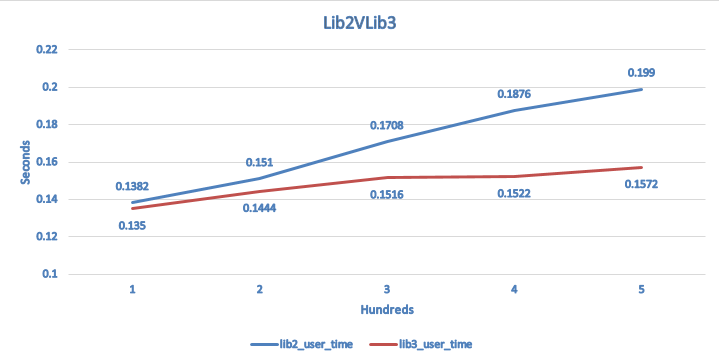
\includegraphics[width=0.7\textwidth]{imgs/compare}
    \caption{Line Chart}
    \label{fig:efficiency line chart}
\end{figure}

